\chapter{$^{294}$Og}
\maketitle

\subsection*{10 April 2017}
Moving on back to working with $^{294}$Og, it would be nice to do calculations with multiple EDFs as a sort of gauge on uncertainties. For Gogny and UNEDF functionals, pairing is included automatically because it was explicitly included in the parameter fit. This is not the case in general, however. So if we want to use SkM*, for instance, we should figure out ahead of time what the pairing interaction will look like. Nicolas and Witek suggested a couple of ways of doing this. Nicolas suggests using experimental mass evaluations to compute binding energies and then the pairing gap, and I assume we can use a formula like this BCS formula to compute the pairing strength from there:
\begin{equation}
\Delta_{BCS} = (E_{max}-E_{min})e^{-\frac{1}{V_0\rho}}
\end{equation}

\noindent where $(E_{max}-E_{min})$ is the spread of single-particle energies for orbitals participating in the pairing (probably taken to be about 60-100 MeV), $\rho = \frac{dn_s}{dE} \approx \frac{A}{100} MeV^{-1}$ is the energy density of states, and $V_0$ is the pairing strength. This should be done for both protons and neutrons. Here is the pairing gap for neutrons (there is not enough data for protons):

\begin{verbatim}
********************************************************************************
*                                                                              *
*  EXTRACTED EXPERIMENTAL PAIRING GAPS, BCS-EQUIVALENT GAPS  AND S.P. LEVELS   *
*                                                                              *
********************************************************************************
*                                                                              *
*  Z =118 **********************************************************************
*                                                                              *
* NEUT DELTA3  DEMINU  DEMIDD  DEPLUS  ESINGP  SEPAR1  SEPAR2  BIND.-EN  ERROR *
*                                                                              *
*?176  0.4410  0.0090  0.4455  0.8820  0.0000  -7.665   0.000 -2078.045 0.5880 *
********************************************************************************
\end{verbatim}

\noindent When all is said and done, you should get something in the ballpark of -250 MeV or so, plus or minus probably like 50 MeV. I think one of those approximations must be wrong somewhere because the numbers I'm getting are nowhere close. Anyway, I'll put that on hold for a moment because we don't have the proton data anyway.

Witek suggests a better way would be to use the inertia-like quantity in equation 4 of \verb|https://journals.aps.org/prl/pdf/10.1103/PhysRevLett.116.152502|. Again, we'd run into the problem of not having enough datapoints nearby, plus I'm also not sure how we'd use this to extract a pairing strength. The paper gives an expression of pairing energy in equation 2, and another way of computing it in this presentation from Nobuo:

\noindent\verb|https://public.ornl.gov/conferences/ns2016/3_Wednesday/Session_1/NS2016_W1_3_Nobuo_Hinohara.pdf|.

\noindent but still no way to relate to the pairing strength, unless you make assumptions about the pairing interaction (like making it only a surface pairing interaction).

\subsection*{18 April 2017}
After talking to Nicolas about it the other day, I guess the best way to find the pairing strength given the pairing gap is actually to just try several different pairing strengths in your input file, and then run them until you get the pairing gap you were hoping for (same goes for whatever quantity it was Witek wanted us to compute). This might involve several HFODD runs for several different nuclei, but it's algorithmic enough that you could make that happen automatically by automating it somehow. Anyway, we'll just leave that up to Jhilam since he's doing the SkM* stuff and I'll take care of UNEDF1-HFB.

\subsection*{3 May 2017}
Here are some observations about the ongoing PES's that I have up to this point:
\begin{enumerate}
\item Symmetric fission has an initial barrier blocking it, but if the nucleus tunnels through (or even wraps around) the barrier, it seems to go to lower energies faster. However, it still seems to scission asymetrically at lower elongations than symmetrically.
\item I'll have to look at the actual outputs or something, but it seems like perhaps triaxiality is reinstated at the first sign of scission around $Q_{20}\approx200$. At this point, it seems likely that whatever scission takes place would probably have a large mass-asymmetry (that's not clear to me from the Q20-Q22-Q30 plot, however).
\item When I started my Q20-Q22 run, I used restart files corresponding (I think) to Q30=4. The result is that in the region between roughly Q20=75 and Q20=125, there is a strong tendency for the system to move to greater mass asymmetry (it'll follow the asymmetric fission valley in your Q20-Q30 plane). After the ridge dividing symmetric and asymmetric paths instersects with the line Q30=4 (which happens at around Q20=125), it will tend back towards symmetric configurations.
\begin{enumerate}
\item The first thing I'd like to do is investigate mass asymmetry for larger quadrupole deformations. I notice there continues to be some octupole activity beyond Q20=125 and I don't know if that is an artifact of which points I used to restart HFODD or if that's just what the surface looks like. Just from checking the output file of Q20=152, Q22=12, it \textit{looks} like it started from the Q20=152, Q30=4 file - and NOT Q20=120, Q22=12 - but I'd like to just be sure, I guess.
\item I'm torn on whether or not to fix the octupole moment to zero, or just to initialize from rec files with Q30=0 and let it evolve from there (it probably won't change at all, in practice, but that's not my decision!). I think I WON'T fix it...
\end{enumerate} 
\end{enumerate}

\subsection*{5 May 2017}
Re: Changing Q30 and seeing how that affects triaxility in Q22 - I restarted an HFODD calculation using mass-symmetric  restart files. For the most part, the outputs all preserved Q30=0 (or almost zero), which is kind of what I expected. The consequential PES shows mostly the same structure as before, with the exception of that region between Q20=75 and Q20=100, where the system must decide whether it will tunnel through the barrier to achieve symmetric fission, or whether to follow the valley towards asymmetric fission. It seems to be energetically favorable in this region for the system to choose mass asymmetry (I just picked the point Q20=100, Q22=2 at "random" and the EHFB difference was something like 2 MeV). I'm thinking the right thing to do now, actually, might be to do another calculation, where this time restart files are chosen from the fission valley. The way I did it the first time was to start everything from the entire line Q30=4, thinking that the system would be free to explore all values of Q30. I was partly right, especially for the values below Q20=75. But once it got over that barrier, Q30=4 is actually \textit{inside} the barrier, leading toward symmetric fission. Those higher Q20 deformations never got the chance to explore higher Q30 values because there was a barrier in the way.

In other news, I discovered a bug in my Python PES plotting script. Whenever I would plot a multipole moment on the z-axis, I would have it subtract the minimum value from all of the other values, in essence shifting the origin from 0 to \texttt{Z0\_min}. That can be helpful for getting a sense of the relationships between points, but not if you want to compare against an absolute scale. Case in point: for detecting scission, you need to know the location of points for which $Q_N\approx0$. But up to (and including) today, my PES didn't contain any points with $Q_N < 8$. So when I thought I was approaching scission, I was actually approaching $Q_N=8$. I've still got quite a way to go before I reach $Q_N=0$!

\subsection*{8 May 2017}
It looks to me (without a full set of converged results) that triaxiality plays a more important role in the mass-symmetric fission case, whereas in the mass-asymmetric case the system favors axiality. So you need one of those symmetries to be broken, but not both? Interesting...

\subsection*{19 May 2017}

I was just re-reading Nicolas' first fission review article (PRC 90.054305.2014), trying to find some significance to the fact that $^{294}$Og reaches its outer turning point so quickly and yet takes a \textit{reeeally} long time to fission (in terms of multipole deformations, that is, and compared to $^{240}$Pu; its half-life is actually probably pretty short because it reaches that outer turning point really quickly and it doesn't have a second minimum fission isomer like $^{240}$Pu). And I noticed a comment about cluster radioactivity in actinides, which upon further investigation is sort of an intermediate between fission and alpha decay, and which tends to leave behind $^{208}$Pb or something close to it. For $^{294}$Og, that would leave the additional daughter fragment $^{86}$Kr, which is semi-magic with 50 neutrons. And HOLY CRAP that's exactly what we get! The only region of my PES that seems to have scissioned so far is exactly that! It's a Christmas miracle!

\subsection*{9 June 2017}

I still won't get to this for a while yet, but I wonder about the formula for the half-life. I know that's one of the most sensitive fission observables. Particular I wonder about the number of assaults on the fission barrier. That's typically taken to correspond to the vibrational energy 1MeV, which is probably a decent estimate but still something that could change depending on your nucleus and configuration. So I would suggest - at the very least - playing around with this number, just to check the robustness of your results before sending them in.

\subsection*{7 August 2017}

Just to update: I'm making progress on the 4D calculations. I had to cheat a little bit to get the constrained dynamical pairing correlations to work (by manually fixing it in the code and recompiling it each time I need a different number), but that seems to be resolved now so that's good. Restarting from $\lambda=0.0$, I got about 1070 points to converge for $\lambda=0.2$ with only about a seven or eight that aborted, and 948 for $\lambda=0.4$ ... The $\lambda=0.2$ calculations should finish pretty quickly based on where their convergence left off; the $\lambda=0.4$ might take a bit longer. I'm going to try the $\lambda=0.15$ set now just to see how quickly those converge, taking the $\lambda=0.2$ record files from which to restart. I'm also going to try starting $\lambda=0.5$ and $\lambda=0.6$ from the $\lambda=0.4$ record files because I think that'll help a bit (though not as much as the $\lambda=0.15$). I'm not sure exactly how high to go in $\lambda$... I think Jhilam said something about that once upon a time? Yes: you just have to check whether the min-action path touches the boundary (in $\lambda$) or not. I'll stop it at $\lambda=0.5$ and check (they didn't need more than $\lambda=0.5$ for $^{240}$Pu, but they went higher for $^{238}$U).

\subsection*{6 September 2017}
I'm trying to understand what would be making it so difficult for the DFT solver to handle the mass symmetric configurations of $^{294}$Og beyond about 500 barns, but not so much the mass asymmetric ones around $(Q_{20},Q_{30})=(600, 90)$. Witek suggests it might be a collapse of pairing, but I'm looking at the pairing gaps and pairing energies and it doesn't appear to be anything like that, since the pairing energies do not disappear. 

\subsection*{15 September 2017}
Last week after talking with Witek, I put together a test run in the subfolder \texttt{.../Q30/pair\_test/}, where I turned on Lipkin-Nogami (but not really; I just used it for the dynamical pairing) with a fixed value of $\lambda_2=0.001$. A couple of my test points converged (and fairly quickly, too, though I'm not sure whether I had tried to make them converge before or not. Probably yes), but the rest diverged.

I was looking back at my Google Keep notes yesterday from a few months back, and I saw basically the same issue with Witek suggesting a similar solution. There, he had suggested using a fixed pairing gap once the pairing gap dropped beneath 400 keV, which is indeed what has happened for the neutrons in some of this region. So I am retrying the points in \texttt{pair\_test} (with the two which converged replaced by two more nearby points). Except this time, instead of using Lipkin-Nogami with a fixed $\lambda_2$ (which, in hindsight, may have also been a bit too large), I'm fixing $\Delta_N=0.5$ (still letting $\Delta_P$ go free, since it was in no danger of disappearing in that region).

I am curious, though: based on this particular PES, there are a surprising number of times when $\Delta_N$ and $\Delta_P$ vary inversely (one goes up while the other goes down). Is there a reason for this? Does it happen in other nuclei?

\begin{adjustwidth}{1cm}{}
$\rightarrow$\quad I can't get the parser to work properly, but my impression is that a similar thing happens in $^{176}$Pt. Not for every point, mind - there are clearly some where the proton and neutron pairing gap is similar. But there are also plenty of cases where they are even different \textit{signs}\dots which feels wrong, actually. So I dunno.
\end{adjustwidth}

\subsection*{19 September 2017}
I did my calculation a few months ago with the finite differences spacing to see how it would affect the inertia. I knew the effect was somewhat large, but I did the tests on $^{240}$Pu originally, which scales differently than $^{294}$Og (so, for instance, a quadrupole moment spacing of 4 barns for plutonium is very different than a quadrupole moment spacing of 4 barns for oganesson). Witek was convinced that the spacing in my oganesson PES should be good enough to compute the inertia accurately as is but I wasn't convinced, based on my plutonium tests. So I ran a test point with a much finer spacing to compare to the coarse PES spacing that I already have. Only one of the coordinates has worked so far (because of a bunch of dumb reasons of things and me being dumb), and I was surprised to see how different the results were: 1.007517E-0002 for the fine spacing versus 1.745241E-0002 for the coarse grid. It's bad enough that I want to check the other coordinates again just to make sure.

\subsection*{25 September 2017}
\textbf{Re: 15 Sept 2017} There was no direct indication in the output files that the neutron pairing gap had been constrained to any particular value. Furthermore, all 9 of my test points diverged. Which, actually, may have been a sign of a constrained pairing gap after all: $\Delta_N$ suddenly tried to jump from like $0.1$ MeV to $0.5$ MeV. I could see how that might lead to a chaotic divergence. It might be preventable with a smooth application of the constraint, but I don't have a clear, simple way of doing that. Nor do I think the problem is so simple, because the pair gap values that the solution jumps between are nowhere near the requested value (nor are they so small as to create the problem Witek was suggesting).

\subsection*{26 September 2017}
I'm trying the same points as yesterday, except instead of fixing the pairing properties, I'm letting them go free and fixing triaxiality. It'll run for a few minutes with just a small triaxial push, after which it should release and go  settle into something more permanent. I only gave it a small triaxial bump because I didn't want to perturb the system so badly it would no longer resemble the restart file (almost a guaranteed convergence failure), but it's entirely possible I might miss a barrier and just slide back down where we started.

\subsection*{28 September 2017}
Something else I did was to look at the cluster decay fragments ($^{208}$Pb and $^{86}$Kr), and compare them to the prefragments using the NLF Chunli developed. It looked pretty much the same, honestly, which is good. But one thing I noticed that I hadn't noticed before is that the shape of the proton spatial localization was very different than the shape of the neutron localization, even for the same nucleus ($^{86}$Kr) at the same deformation. I asked Witek if this was evidence for a collective excitation where the protons and neutrons undergo some quadrupole vibration independently of one another, and he said yes. The word he used, I believe, was ``isovector vibration'' or something like that. So that's a word I need to learn, but at least it seems like a good result!

\subsection*{29 September 2017}
Studying up some more on cluster emission, I decided to look back at some of my other localization plots to see if there was any evidence of shell formation early on in the trajectory. And sure enough, you can see evidence of shell formation of both the krypton and the lead in the neutron spatial localization as far back as the outer turning point, which is when I started storing my localization files. You can also see a proton shell starting to form in the lead, but it's not so clear in the krypton. This kind of makes sense, I guess: $^{86}$Kr has a magic number of neutrons but not protons, while $^{208}$Pb is magic in both neutron and proton numbers.

\begin{figure}[h!]
  \begin{center}
    \subfigure[$Q_{20}=140 b, Q_{30}=24 b^{\frac{3}{2}}$\newline (just beyond the outer turning point)]{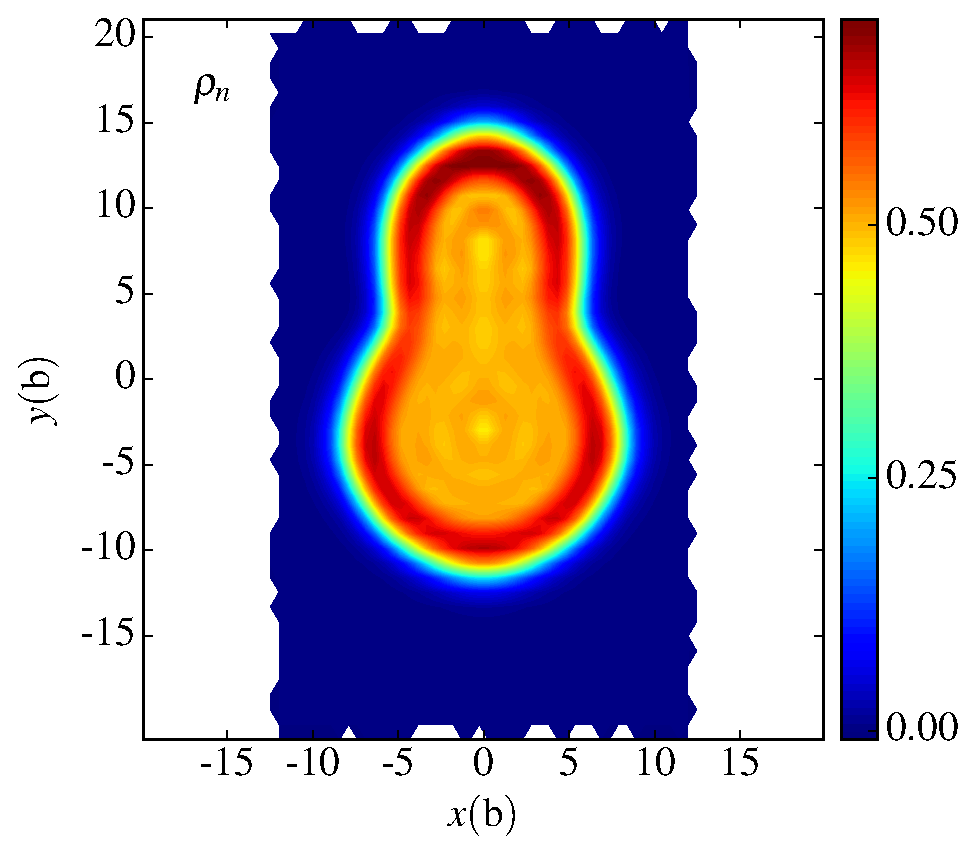
\includegraphics[width=0.3\linewidth]{294Og-140024n-locali.eps}}\label{fig:294Og-140024n-locali}
    \subfigure[$Q_{20}=200 b, Q_{30}=44 b^{\frac{3}{2}}$]{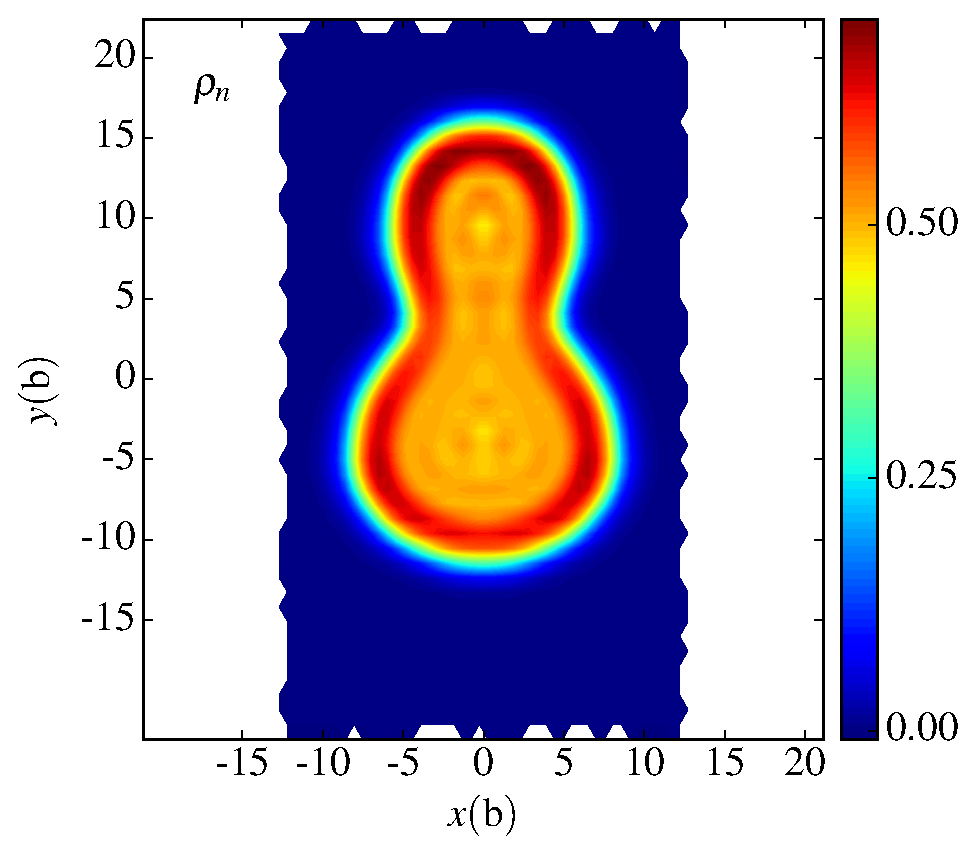
\includegraphics[width=0.3\linewidth]{294Og-200044n-locali.eps}}\label{fig:294Og-200044n-locali}
    \subfigure[$Q_{20}=264 b, Q_{30}=60 b^{\frac{3}{2}}$\newline (just before scission)]{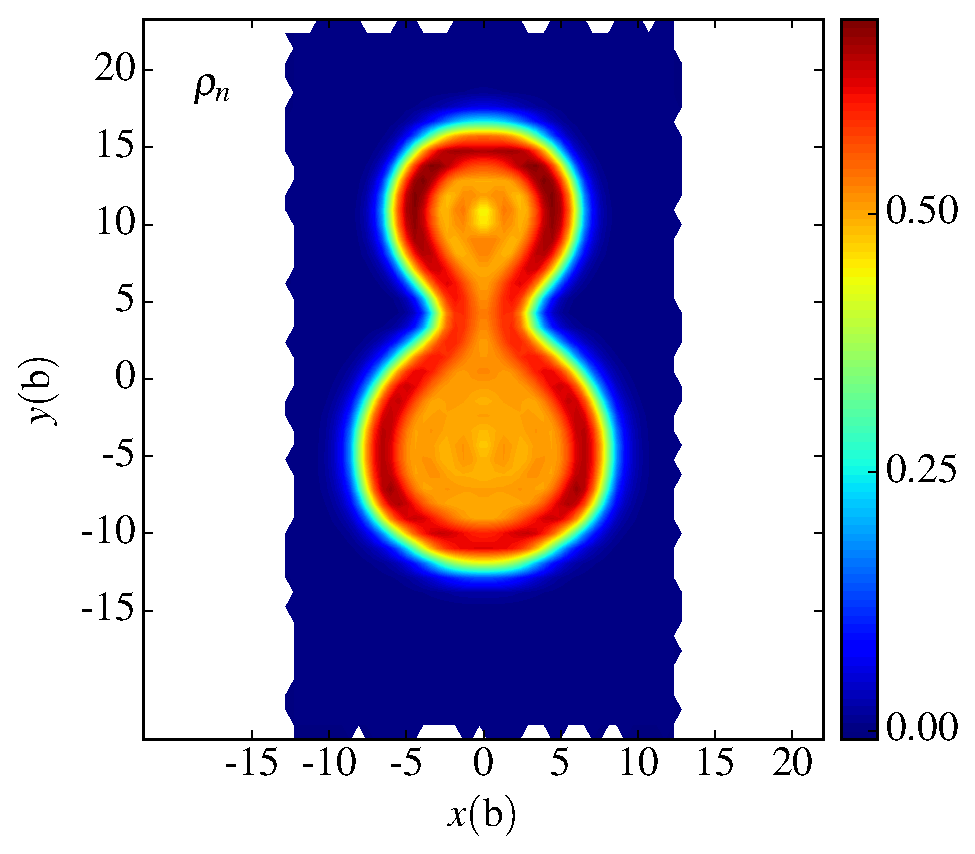
\includegraphics[width=0.3\linewidth]{294Og-264060n-locali.eps}}\label{fig:294Og-264060n-locali}  \end{center}
  \caption{Neutron spatial localization for $^{294}$Og. Shells are already starting to develop as early as just beyond the scission point}

%\end{figure}
%
%\begin{figure}[h!]
  \begin{center}
    \subfigure[$Q_{20}=140 b, Q_{30}=24 b^{\frac{3}{2}}$ (just beyond the outer turning point)]{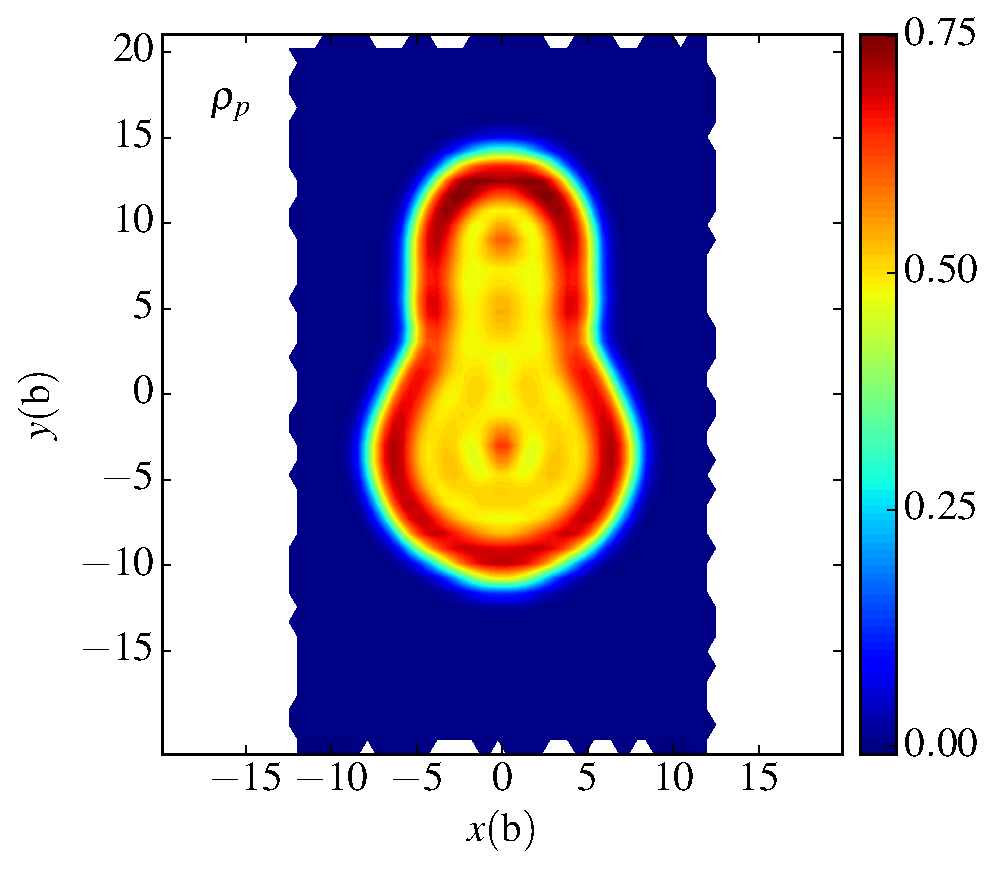
\includegraphics[width=0.3\linewidth]{294Og-140024p-locali.eps}}\label{fig:294Og-140024p-locali}
    \subfigure[$Q_{20}=200 b, Q_{30}=44 b^{\frac{3}{2}}$]{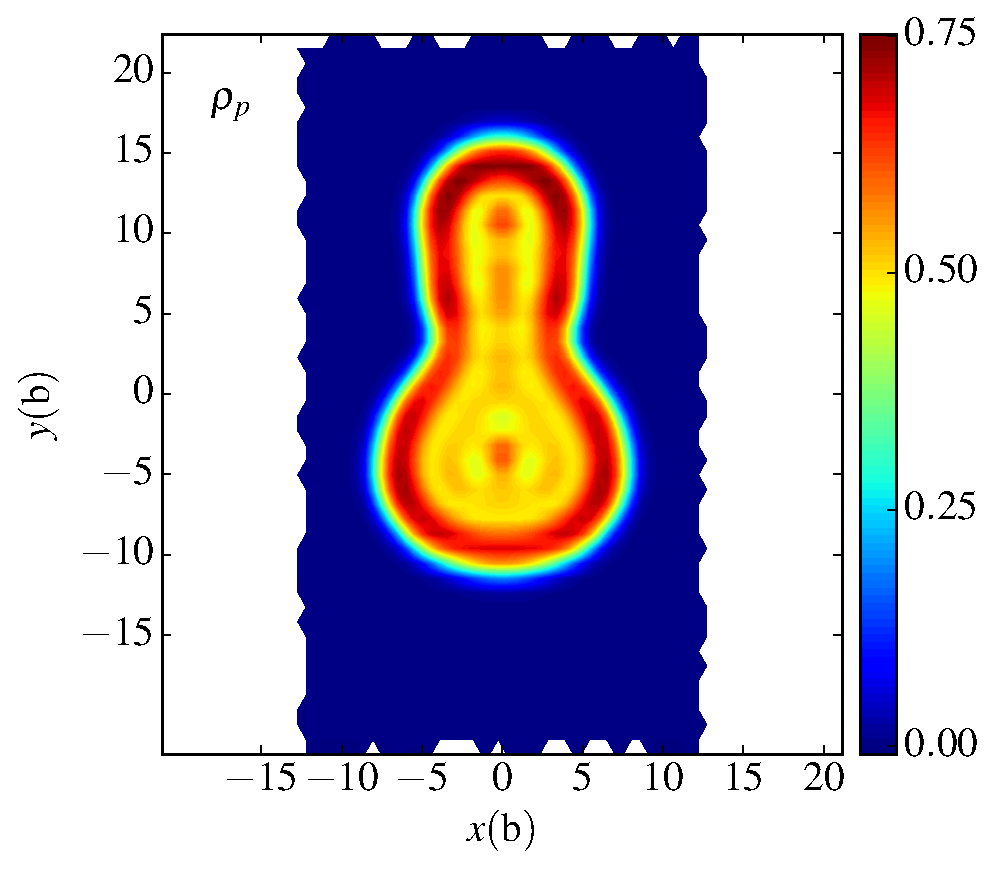
\includegraphics[width=0.3\linewidth]{294Og-200044p-locali.eps}}\label{fig:294Og-200044p-locali}
    \subfigure[$Q_{20}=264 b, Q_{30}=60 b^{\frac{3}{2}}$ (just before scission)]{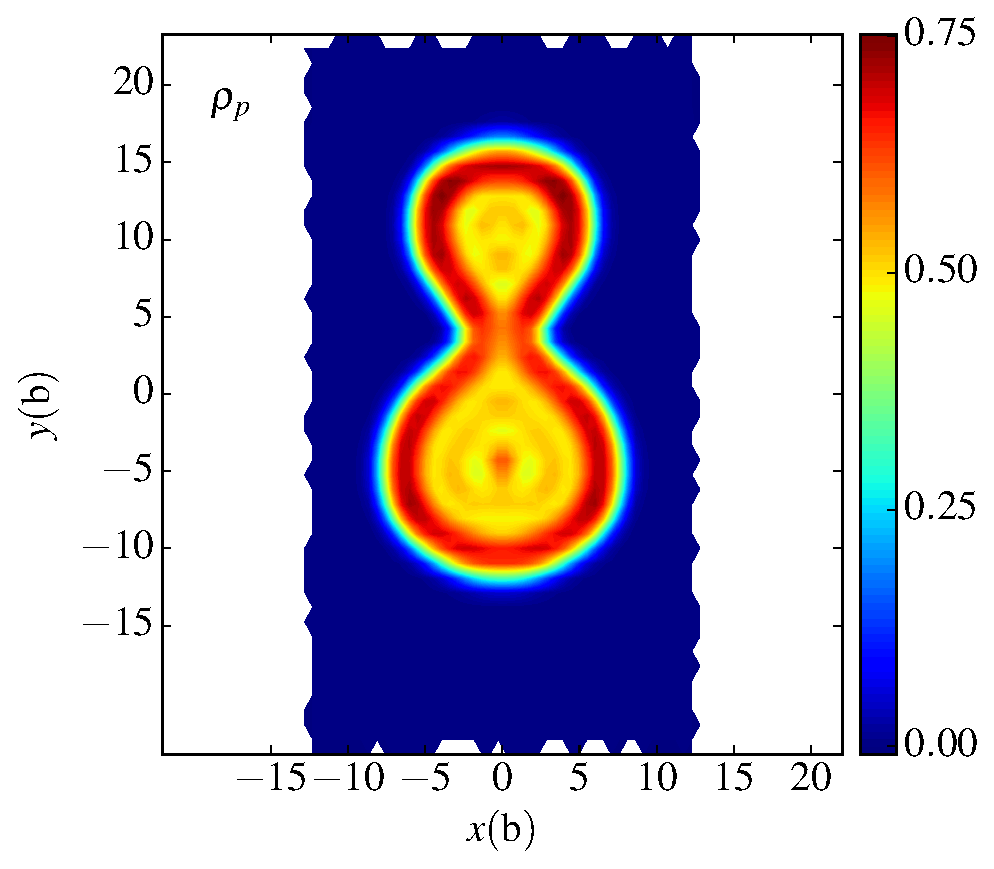
\includegraphics[width=0.3\linewidth]{294Og-264060p-locali.eps}}\label{fig:294Og-264060p-locali}  \end{center}
  \caption{Proton spatial localization for $^{294}$Og. Note that the lead proton shell starts to develop early, but the krypton proton shell doesn't develop until much later}
\end{figure}

\subsection*{2 October 2017}
One more comment I want to make clear about the plots from the previous entry: some models of cluster emission treat the system as a preformed smaller fragment trying to escape from the larger fragment. What these plots seem to show is almost the opposite, where you have a well-formed core trying to shed its excess nucleons.

\subsection*{4 October 2017}
\textbf{Re: 26 September 2017} I got back the results from giving the system a small, triaxial boost. It seems to have worked from a software perspective - they all reported back non-zero values for $Q_{22}$ - but in the end, everything still diverged. Also, it's entirely possible the boost wasn't enough - maybe there's a large triaxial barrier and $Q_{22}=3$ just wasn't enough to make it to the other side. So I guess that's the next thing I'll try. Instead of $Q_{22}=3$, I'm going to try it with $Q_{22}=30$. That might well fail, as well, just because of the jump, but it's something to try, right? And I'll do it with 10 iterations of ``pushing'' instead of 5.

\subsection*{10 October 2017}
Yeah, that large triaxial push was \textit{definitely} too much for it. Maybe if I had eased into it instead of jumping so abruptly that could have done it. But the way I did it (pushing directly from $Q_{22}=0$ to $30$) was just too much and it caused the thing to diverge after only 45 minutes (\texttt{QUABCS failed for neutrons/protons}).

\subsection*{1 December 2017}
Something that we noticed a few weeks ago was that I may have misunderstood what how $\lambda_2$ was chosen in Jhilam's \textit{Pairing-Induced Speedup} paper. I just took $\lambda_2=0$ as my baseline, but Samuel suggests that what I should have done is performed a self-consistent calculation first (with Lipkin-Nogami turned on), and then used whatever $\lambda_2$s came out of that as my baseline/zero/starting point. So now I picked a point ($Q_{20}=48, Q_{22}=15, Q_{30}=6$) and redid it with Lipkin-Nogami to use as a baseline. That converged with some values like $\lambda_{2n}=0.094, \lambda_{2p}=0.118$, which is well-within the range of $\lambda_2$-values I probed. Except that if you go to a larger value of $\lambda_2$, even as small a change as $\lambda_2=0.15$, you end up with a lower HFB energy. And worse, there seems to be a monotonic decrease at least as far as $\lambda_2=0.4$. It might start increasing again by the time I get to $\lambda=0.5$ and beyond - that's certainly what my calculation shows, but I remember being skeptical of that run for some reasons that I can't currently remember. Anyway, so I'm playing around with that, just to see if there's anything going on that we can't see somehow. So for instance, as I said I did an unconstrained calculation kickstarted with HFBTHO; now I'm using that record file to start a run using  $\lambda_2=0.15$ and another with $\lambda_2=0.4$. Hopefully, if the problem relates to the initial conditions (where in the variational space you are looking), that should show us.

UPDATE: I didn't let the two run to complete convergence, because I didn't want to waste resources, but the overall HFB energy for each constrained run at each iteration was significantly lower than the ``self-consistent'' solution, to at least 2 decimal points of precision.

UPDATE 2: Nope, wait, I was being dumb. You maybe weren't totally wrong, per se, but a better idea would be to use a constrained calculation to force yourself into a certain region, and then release the constraint from there. That's what you tried to do in the first place. Here you're just being perhaps a bit more careful about it, hopefully.

\subsection*{5 December 2017}
Okay, I think I did it better this time. I took several points, each with the same multipole constraints ($Q_{20}=45, Q_{30}=12, Q_{22}=0$), and gave them each a $\lambda_2$ in the range $[0.0, 0.9]$ in steps of $0.1$ (and a few in the middle in steps of $0.05$). I ran those and about a quarter of them converged (the other $\frac{3}{4}$ seem mostly to have diverged chaotically). Within that group, the final total energy seems to have decreased monotonically (and it's not clearly from one specific contribution, like for example the Lipkin energy). Granted, the three that converged were the three with both the smallest value of $\lambda_2$ and the ones closest to the self-consistent solution's preferred value of $\lambda_2$; perhaps if the others had managed to converge we would have seen a minimum in the final energy, followed by an increase somewhere. But given the results I have, and the range I have, there is only a decrease in the total energy, not a minimum.

Interestingly, even though some of those points converged, I was able to take their unconverged record files and run them alongside the converged record files to let the system run to its true self-consistent solution. Almost everything converged; the few that didn't seem to have gotten stuck in a nearby false minimum. But as there doesn't appear to be a particular pattern dictating which got stuck and which ones didn't, I'm content claiming that the solution from those which converged is a ``global'' minimum.

However, if you subtract off the Lipkin energy from the total energy (see eqn 6.1 in my notes, or roughly I-9, VI-96 in the original HFODD papers), you see that the total energy \textit{before} the Lipkin-Nogami correction bottoms out around the self-consistent minimum value of $\lambda_2$ (of course, there will also be a slightly different self-consistent minimum if you run the code without Lipkin-Nogami or dynamical pairing [$\lambda_2=0$]).

\subsection*{5 February 2018}
It's been a while since I wrote, but I've got some things worth recording.

As far as I can tell, I have a minimum-action pathway/half-life code that seems to do a reasonably-good job finding minimum action pathways, but a less good job finding half-lives. It still isn't a totally-settled deal - one thing we can adjust is the zero-point energy or the energy of the ground state. Changing the $E_0$ which appears in the action integral by something like 0.1 MeV can alter the half-life by a factor of like 2 or 4 (depending which way you go). Not enough to account for my results, unfortunately, but something (and actually, in the case of oganesson, it might change my results in the opposite direction to what I need).

One problem we encountered was that we were getting $M_{eff}<0$ at some points, which is of course ridiculous! Presumably these points correspond to some kind of level crossing between points on the potential energy surface (recall that components of the inertia tensor were computed using finite differences). There are probably a number of ways I could have resolved the issue (apparently Jhilam just replaced the negative values with zeros, which makes me just a little uncomfortable), but I settled on writing a Python script that checked the value of $M_{eff}$ along each possible direction (as determined by the action minimization code using chiefly the parameters \texttt{b\_span} and so on). If a point has $M_eff\geq0$ along every possible trajectory, it is rewritten into a new, filtered input file; otherwise it is discarded. This unfortunately eliminates roughly $\frac{3}{4}$ of the data I collected. I can still use my full interpolated PES by running the code first using the unfiltered input file, saving \texttt{EHFB\_int.out}, and using it to jumpstart the next run, but unfortunately a lot of that inertia data is simply lost to time. It might be worth seeing which points I do manage to keep, in order to know if my subsequent inertia is reasonable or not. That would be a good thing to check.

In any case, using the inputs as presently constituted, I computed the half-life (and the pathways) in 2-, 3-, and 4-D space using the collective coordinates $(((q_{20},q{30}),q_{22})\lambda_2)$. The results I get currently are:

\begin{list}{}{Half-lives in 2, 3, and 4 dimensions:}
\item 2D $(q_{20},q_{30}); q_{22}=3, \lambda_2=0$:    1305504.9263348267     
\item 3D $(q_{20},q_{30},q_{22}); \lambda_2=0$:    3.8268163795048664E+022
\item 3D $(q_{20},q_{30},\lambda_2); q_{22}=3$:    9.4084322399806967E-012
\item 3D $(q_{20},q_{22},\lambda_2); q_{30}=0$:    4.9637739301242774E-011
\item 4D $(q_{20},q_{30},q_{22},\lambda_2)$:       3.8820411419017089E-012
\end{list}

\subsection*{6 February 2018}
I plotted the inertias that made it through the filter (in particular, in the 3D case). There's enough to capture sort of the bulk properties of the PES, but it depends on which layer (which value of $q_{22}$) you're looking at. The parts that I'm most worried about are probably the barrier(s), and you can kind of see them but not in any clear detail. Is that enough? I dunno. I don't even know what that means...
\begin{figure}
\centering
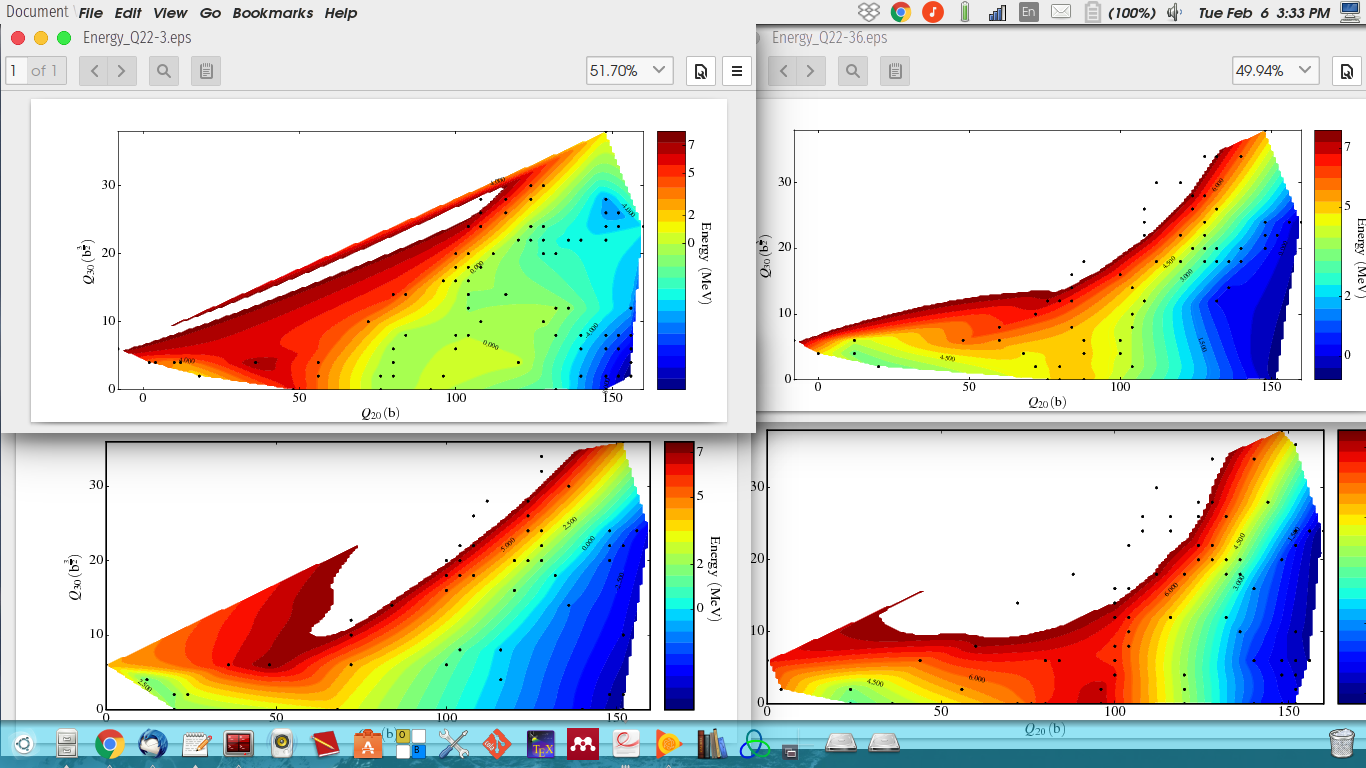
\includegraphics[width=0.9\linewidth]{post_filtering_nans}
\caption[Points with $M_{eff}>0$]{Points with $M_{eff}>0$ (and all NaNs filtered out) shown for several values of $q_{22} (q_{22}=3,24,36,45)$}
\label{fig:post_filtering_nans}
\end{figure}

\subsection*{7 February 2018}
My abs are so sore! But that's not relevant...

I did the 4D path calculation again, but this time I added/subtracted 100 keV to the ground state energy in the action integral to see the effect on the half-life. Pretty much as expected, but now I know. The problem, though, (and as I may have said before) is that my half-life is already too small. Increasing $E_0$ (which is what Witek suggested doing) just makes it smaller.

Just out of curiosity, I also decided to try out my alternative way of computing the tunneling probabilty. That, too, is shown below.

\begin{list}{}{Half-lives with different ground state energies:}
\item $\sqrt{V-E_0-0.1}$:    4.5456834751698960E-013
\item $\sqrt{V-E_0}$:    3.8820411419017089E-012
\item $\sqrt{V-E_0+0.1}$:    1.9654750844481639E-010
\item $\sqrt{V-E_0+0.5}$:    4.8651043198529695E-007
\item Alternative tunneling prob.: Nonsense. It really depends a lot on your choice of $E_{ZPE}$
\end{list}

Also perhaps worth noting is the fact that the minimum action trajectory sometimes changes depending on your ground state energy offset. Most of them claim to stay fairly mass-symmetric and very triaxial (Really? Huh. That's interesting), but there are exceptions.

\subsection*{5 April 2018}
Samuel generated a 2D PES for $^{294}$Og using the Gogny D1M force using a perturbative recipe for the inertia. Using the values he gave me I computed a value for the half-life of Oganesson:

\begin{list}{}{Half-life in 2 dimensions from Gogny:}
\item 2D (no ZPE) $(q_{20},q_{30})$:        30786236776.996628 ($3.1x10^10$)
\end{list}

I'm running into some kind of problem when I try to add in the ZPE, which may owe to the fact that apparently I don't know what the ZPE is after all. Also, when I compared Samuel's input data to my own, I noticed that while $M_{q2q2}$ is of approximately the same magnitude in both cases, the other two components are roughly an order-of-magnitude larger in my file than in his. What's up with that? Did I convert from Fermis to barns wrong with Samuel's data? Or did I do something dumb with my data? Or are the data really just that different?

\subsection*{11 April 2018}
I added a little workaround in order to use ZPE corrections to the ground state (the real fix is going to take a little bit of work, though nothing too terrible). With a ZPE correction of 0.5, I now get:

\begin{list}{}{Half-life in 2 dimensions from Gogny, take 2:}
\item 2D (ZPE=0.5) $(q_{20},q_{30})$:        9837943407.0663910 ($9.8x10^9$)
\end{list}

Sooo... Slightly-better...

Importantly, though, the exit point changes significantly with that correction, though. Before, it was exiting along the symmetric path. But with the added 0.5 MeV correction, it now exits along the cluster path. Interesting...

\subsection*{17 May 2018}
We discovered a problem with my data: that I was using $E_{HFB}+E_{LN}$ instead of just $E_{HFB}$ (or something like that). The issue was (as I describe in my lecture notes) that HFODD subtracts off a correction term corresponding to dynamical pairing correlations and minimizes \textit{this} energy to drag the energy down in a way that corresponds with increased pairing fluctuations, but in order to get the correct answer (at least for what we're doing, which isn't truly a Lipkin-Nogami problem) you would need to remove this energy correction at the very last step before reporting your final energy. I had not done this in my previous runs, so all the half-lives I was getting were artificially small, and the paths were nonsense because they always wound up favoring the configuration with the highest $\lambda_2$. I've corrected this now and reevaluated the minimum action path (and since I had to redo things anyway, I merged the 2D extended axial PES with the 4D limited-region, triaxial PES). That done, here are the half-lives I get:

\begin{list}{}{Half-lives with correct treatment of Lipkin energy}
	\item 4D, dynamic (ZPE=1.0) $(q_{20},q_{30},q_{22},\lambda_2)$:        9.087167283468209e-09
	\item 4D, dynamic (ZPE=1.0), OTL fixed to $q_{22}=\lambda_2=1$ $(q_{20},q_{30},q_{22},\lambda_2)$:        4.438500943515716e-08
	\item 4D, static (ZPE=1.0) $(q_{20},q_{30},q_{22},\lambda_2)$:        6.9109675005e-05
	\item 4D, static, constant $M_{eff}$ (ZPE=1.0) $(q_{20},q_{30},q_{22},\lambda_2)$:        30607.4713611
	\item 2D, dynamic, (ZPE=1.0) $(q_{20},q_{30}), q_{22}=\lambda_2=0$:        441058141967.03418
	\item 2D, static, (ZPE=1.0) $(q_{20},q_{30}), q_{22}=\lambda_2=0$:        3.77931485423e+51
\end{list}

\noindent I can't get a 3D calculation (or not a correct one) using the data I have. Because of the way I did my calculations, if I limit myself to $\lambda_2=0$, then I automatically impose $q_{22}=0$ as well. That's not actually true, but what is true is that I don't have any $q_{22}$ inertias for $\lambda_2=0$ for some reason.
